\documentclass[tikz,border=2pt]{standalone}
\usepackage{tikz}
\usetikzlibrary{arrows.meta,positioning,calc}
\definecolor{ink}{HTML}{1F2933}
\definecolor{line}{HTML}{52606D}
\definecolor{panel}{HTML}{F5F7FA}
\definecolor{network}{HTML}{0E7490}
\definecolor{power}{HTML}{B45309}
\definecolor{store}{HTML}{475569}
\begin{document}
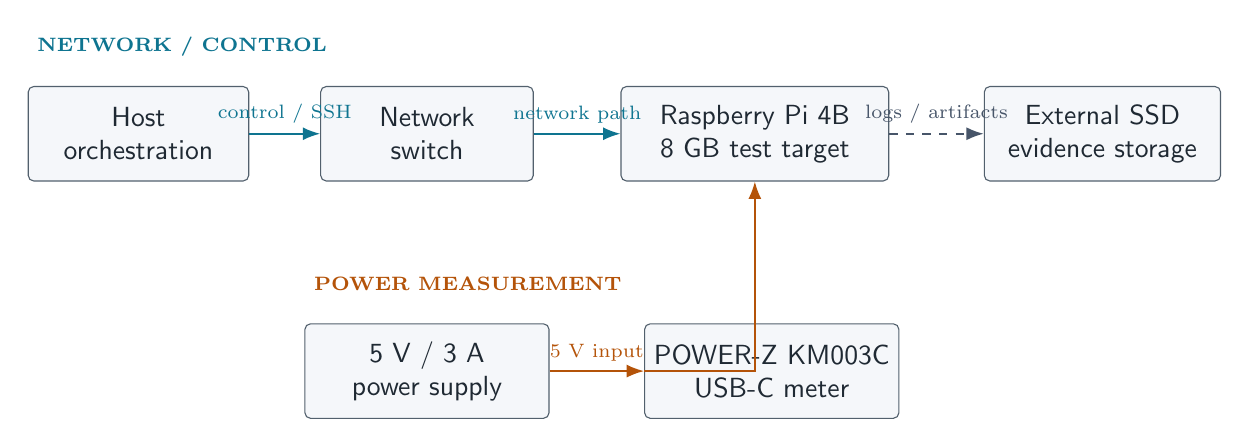
\begin{tikzpicture}[
  font=\sffamily,
  box/.style={draw=line,fill=panel,rounded corners=2pt,minimum height=12mm,align=center,text=ink},
  arr/.style={-{Latex[length=2.2mm]},line width=.65pt},
  lab/.style={font=\scriptsize\bfseries,text=ink}
]
\node[box,minimum width=28mm] (host) {Host\\orchestration};
\node[box,minimum width=27mm,right=9mm of host] (sw) {Network\\switch};
\node[box,minimum width=34mm,right=11mm of sw] (pi) {Raspberry Pi 4B\\8 GB test target};
\node[box,minimum width=30mm,right=12mm of pi] (ssd) {External SSD\\evidence storage};

\node[box,minimum width=31mm,below=18mm of sw] (psu) {5 V / 3 A\\power supply};
\node[box,minimum width=31mm,right=12mm of psu] (meter) {POWER-Z KM003C\\USB-C meter};

\draw[arr,network] (host) -- node[above,font=\scriptsize,text=network]{control / SSH} (sw);
\draw[arr,network] (sw) -- node[above,font=\scriptsize,text=network]{network path} (pi);
\draw[arr,store,dashed] (pi) -- node[above,font=\scriptsize,text=store]{logs / artifacts} (ssd);

\draw[arr,power] (psu) -- node[above,font=\scriptsize,text=power]{5 V input} (meter);
\draw[arr,power] (meter) -| (pi.south);

\node[lab,anchor=west,text=network] at ($(host.north west)+(0,5mm)$) {NETWORK / CONTROL};
\node[lab,anchor=west,text=power] at ($(psu.north west)+(0,5mm)$) {POWER MEASUREMENT};
\end{tikzpicture}
\end{document}
